\section{Tests}
\begin{frame}{Tests}
  Tests based on system responsiveness
  \begin{itemize}
    \item<1-> Docker vs VirtualBox startup
    \item<2-> SFC length startup 
  \end{itemize}
\end{frame}

\subsection{Docker vs Hypervisor-based virtualization}
\begin{frame}{Tests - Docker vs VirtualBox}

  % TODO insert data?
  \begin{figure}
    \centering
    \begin{subfigure}[b]{0.45\textwidth}
      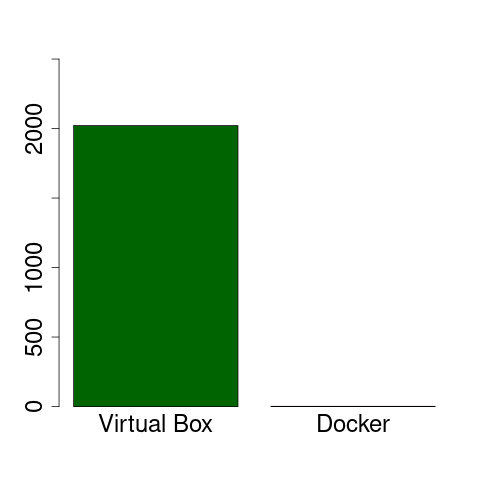
\includegraphics[width=\textwidth]{docker_vs_vmBarplotGraph}
    \end{subfigure}
    ~
    \begin{subfigure}[b]{0.45\textwidth}
      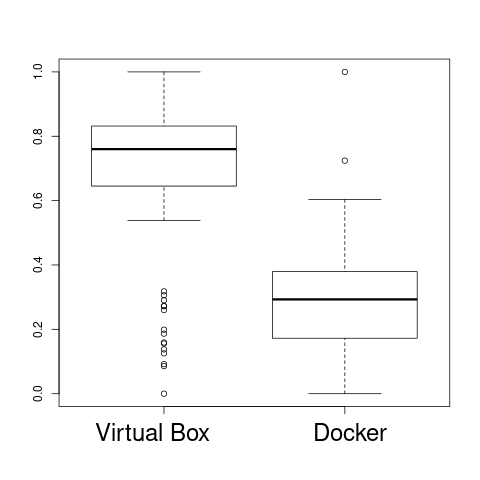
\includegraphics[width=\textwidth]{docker_vs_vmBoxplotGraph}
    \end{subfigure}
  \end{figure}
  \begin{itemize}
  \item Average start up time for Docker: 0.016 seconds
  \item Average start up time for Virtual Box: 20.211 seconds
  \end{itemize}
\end{frame}

\subsection{SFC length startup}
\begin{frame}{Tests - SFC length startup}
  \begin{figure}
    \centering
    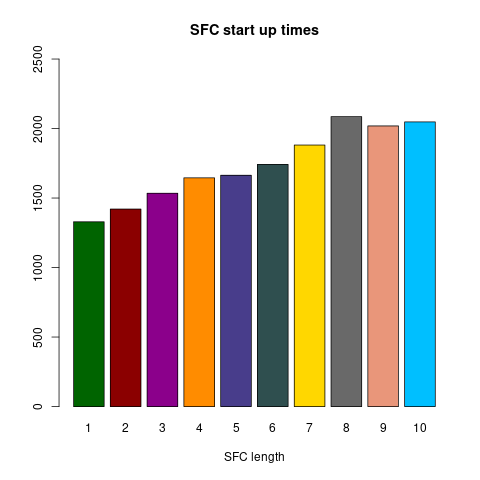
\includegraphics[scale=0.25]{sfc_startupBarplotGraph}
  \end{figure}

  Average start up time (in seconds):
  \begin{multicols}{2}
    \begin{itemize}
    \item 1 element: 13.291 s
    \item 5 elements: 16.634 s
    \item 10 elements: 20.511 s
    \end{itemize}
  \end{multicols}

  \vfill
\end{frame}
